

\newcommand{\pol}{\ensuremath{\pi}}
\newcommand{\optpol}{\ensuremath{{\pol}_\ast}}
\newcommand{\polset}{\ensuremath{\Pi}}
%\newcommand{\curs}{{s_\mathrm{C}}}
\newcommand{\curs}{s}
\newcommand{\cura}{a}
%\newcommand{\nexta}{{a_{N}}}
%\newcommand{\nexts}{{s_{N}}}
\newcommand{\nexta}{{a'}}
\newcommand{\nexts}{{s'}}
\newcommand{\condsetbig}[2]{\left\{\left.#1\right|#2\right\}}
\newcommand{\condprobbig}[2]{p\left(\left.#1\right|#2\right)}
\newcommand{\Condprobbig}[2]{P\left(\left.#1\right|#2\right)}
\newcommand{\df}{\gamma}
\newcommand{\condprobb}[2]{p(#1|#2)}
\newcommand{\suppk}[1]{\ensuremath{\mathcal{#1}}}
\newcommand{\suppx}{\suppk{X}}
\newcommand{\suppy}{\suppk{Y}}
\newcommand{\suppz}{\suppk{Z}}
\renewcommand{\Expect}{\mathbf{E}}

\newcommand{\stateset}{\ensuremath{\mathcal{S}}}
\newcommand{\actionset}{\ensuremath{\mathcal{A}}}

\newcommand{\assign}{\leftarrow}


The reinforcement learning is a machine learning where an agent learns how to take actions to achieve a goal
by maximizing cumulative reward while interacting with environment.
Learning from interaction is a foundational idea underlying nearly all theories of learning and intelligence.

It differs from supervised learning in that labeled input and output pairs need not be presented
(and sub-optimal actions need not be explicitly corrected).
Instead the focus is finding a balance between exploration of uncharted territory and exploitation of current knowledge.
It is much more focused on goal-directed learning from interaction than other approaches to machine learning.

Here we primarily explore idealized learning situations and evaluate the effectiveness of various learning methods.


\section{Finite Markov Decision Processes}

We introduce the formal problem of finite Markov decision processes (MDPs),
which we try to solve.
This problem involves evaluative feedback,
but also an associative aspect, \ie, choosing different actions in different situations.
MDP is a classical formalization of sequential decision making,
where actions influence not just immediate rewards,
but also subsequent states through those future rewards.
Thus MDPs involve delayed reward and the need to trade-off immediate and delayed reward.

\figurename~\ref{fig:mdp} depicts MDP where an agent interacts with environment.
The current state of the environment is known to the agent.
With knowledge of state, the agent makes a decision as to which action to take.
This action, in turn, will change the state of the environment and the agent will receive
a reward at the same time.
The agent remembers this reward in some indirect way and uses it for making future decisions.

\begin{figure}
\begin{center}
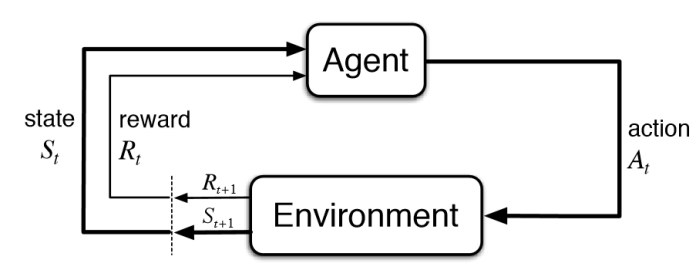
\includegraphics[width=.7\textwidth]{figures/reinforcement-learning}
\end{center}
\caption{The agent-environment interaction in a Markov decision process.}
\label{fig:mdp}
\end{figure}


\subsection{Markov property}


Suppose that the agent is in state $S_t$ takes action $A_t$ at time $t$.
Then the agent receives reward $R_{t+1}$ (from the environment) and the environment transitions to state $S_{t+1}$.
MDP assumes that all these quantities are random variables.

Let \stateset\ and \actionset\ be the set of all the states and that of all the actions the agent can take respectively.

Now suppose that the environment is in state $S_0\in\stateset$ the agent takes action $A_0\in\actionset$ at $t=0$.
Then the state of the environment becomes $S_1\in\stateset$ giving the agent $R_1\in\reals$ as reward.
Suppose that the agent repeat taking actions.

Then we have a sequence of random variables
\begin{equation}
S_0, A_0,
R_1, S_1, A_1,
R_2, S_2, A_2,
R_3, S_3, A_3,
\ldots
\end{equation}

We assume that these random variables satisfy the Markov Property (as assumed by the name) in the following sense.

\begin{equation}
S_{t+1}, R_{t+1} | S_{t}, A_{t}, R_{t}, S_{t-1}, A_{t-1}, R_{t-1}, \ldots
= S_{t+1}, R_{t+1} | S_{t}, A_{t}
\end{equation}
\ie, two random variables, $S_{t+1}$ and $R_{t+1}$, conditioned on every state, action, and reward before $t+1$
are the same as those conditioned on $S_t$ and $R_t$ only.

This can be formally expressed using the probability density function (PDF)
as follows.
\begin{equation}
\condprobbig{S_{t+1}, R_{t+1} }{ S_{t}, A_{t}, R_{t}, S_{t-1}, A_{t-1}, R_{t-1}, \ldots}
= \condprobbig{S_{t+1}, R_{t+1} }{ S_{t}, A_{t} }.
\end{equation}

This is the reason that the process is called \emph{Markov} decision process.

\subsection{Policy}

The \emph{policy} is defined by the conditional probability of $A_{t}$ given $S_{t}$,
\ie,
\begin{equation}
\pol(A|S) = \condprobb{A_t}{S_t},
\end{equation}
which implies the probability of taking certain action depends only on the current state, not the time.
The policy decides which actions the agent takes in each state.

Let \polset\ be the set of all the policies.

\subsection{Return}

The \emph{return} at $t$ is defined by
\begin{equation}
        G_t
        = \sum_{k=0}^\infty \gamma^k R_{t+k}
        = R_{t+1} + \gamma R_{t+2} + \gamma^2 R_{t+3} + \cdots
\end{equation}
where $\gamma \in [0,1]$ is called the \emph{discount factor}.
If $\gamma=0$, the agent is myopic, \ie, it only cares the immediate reward.
If $\gamma=1$, the agent is truly far-sighted, \ie, it cares all the future rewards without discounting.
If $\gamma$ is somewhere between $0$ and $1$, it considers near-future rewards more importantly than those in far future.


\subsection{State value function and action value function}

The state value function (which is sometimes referred to as just value function) is defined by
\begin{equation}
v_\pol(\curs)
= \Expect_{\pol,p} \condsetbig{G_{t}}{S_t = \curs}
= \Expect_{\pol,p} \condsetbig{
    \sum_{k=0}^\infty \gamma^k R_{t+k}
    }{S_t = \curs}.
\end{equation}
In other words, the state value function is a function of a state
representing the expected return the agent will get from the state
when following the policy $\pol$.

The action value function (which is sometimes referred to as just action function) is defined by
\begin{equation}
q_\pol(\curs, \cura)
= \Expect_{\pol,p} \condsetbig{G_{t}}{S_t = \curs, A_t = \cura}
= \Expect_{\pol,p} \condsetbig{
    \sum_{k=0}^\infty \gamma^k R_{t+k}
    }{S_t = \curs, A_t = \cura}.
\end{equation}
In other words, the action value function is a function of a state and an action
representing the expected return the agent will get from the state when the agent takes a certain action
and follows the policy $\pol$.

As mentioned above, most reinforcement learning algorithms try to maximize either one of these functions,
\ie,
not maximizing the immediate reward, but the long-term return.

\newpage
\section{Bellman equation}

\href{https://en.wikipedia.org/wiki/Richard_E._Bellman}{Richard E. Bellman}, who introduced dynamic programming in $1953$,
proposed an equation as a necessary condition for optimality associated with dynamic programming,
which is called Bellman equation.
One of the properties that Markov property implies is that the value functions only depend on the current state (and the action taken)
and that the function value is closely related to the function values of the next states.
These facts are cleverly used to derive the Bellman equation.
Here we introduce two Bellman equations; one for the state value function and the other for action value function.

To derive Bellman equations, we use some basic statistics facts regarding conditional expectations.
(Refer to \S\ref{sec:rl-app}.)

Since the definitions of state value function and action value function together with (\ref{eq:dkci}) imply
\begin{eqnarray*}
v_\pol(\curs)
&=& \Expect_{\pol,p} \condsetbig{G_{t}}{S_t = \curs}
\\
&=& \Expect_{A_t|S_t =\curs} \Expect_{\pol,p} \condsetbig{G_{t}}{S_t = \curs, A_t}
\\
&=& \sum_\cura p(A_t=\cura|S_t =\curs) \Expect_{\pol,p} \condsetbig{G_{t}}{S_t = \curs, A_t=\cura}
\\
&=& \sum_\cura \pol(\cura|\curs) \Expect_{\pol,p} \condsetbig{G_{t}}{S_t = \curs, A_t=\cura}
\\
&=& \sum_\cura \pol(\cura|\curs) q_\pol(\curs,\cura)
\end{eqnarray*}
and
\begin{eqnarray*}
q_\pol(\curs, \cura)
&=& \Expect_{\pol,p} \condsetbig{G_{t}}{S_t = \curs, A_t = \cura}
\\
&=& \Expect_{S_{t+1}, R_{t+1}|S_t=\curs,A_t=\cura} \Expect_{\pol,p} \condsetbig{G_{t}}{S_t = \curs, A_t = \cura, S_{t+1}, R_{t+1} }
\\
&=& \Expect_{S_{t+1}, R_{t+1}|S_t=\curs,A_t=\cura} \Expect_{\pol,p} \condsetbig{\sum_{k=0}^\infty \df^k R_{t+k+1}}{S_t = \curs, A_t = \cura, S_{t+1}, R_{t+1} }
\\
&=& \Expect_{S_{t+1}, R_{t+1}|S_t=\curs,A_t=\cura} \Expect_{\pol,p} \condsetbig{R_{t+1} + \df \sum_{k=0}^\infty \df^k R_{t+k+2}}{S_t = \curs, A_t = \cura, S_{t+1}, R_{t+1} }
\\
&=& \sum_{\nexts, r} p_{S_{t+1}, R_{t+1}|S_t,A_t}(\nexts, r|\curs,\cura) \Expect_{\pol,p} \condsetbig{R_{t+1} + \df G_{t+1} }{S_t = \curs, A_t = \cura, S_{t+1} = \nexts, R_{t+1} =r}
\\
&=& \sum_{\nexts, r} p_{S_{t+1}, R_{t+1}|S_t,A_t}(\nexts, r|\curs,\cura) \left( r + \df \Expect_{\pol,p} \condsetbig{G_{t+1}}{S_t = \curs, A_t = \cura, S_{t+1} = \nexts, R_{t+1} =r} \right)
\\
&=& \sum_{\nexts, r} p_{S_{t+1}, R_{t+1}|S_t,A_t}(\nexts, r|\curs,\cura) \left( r + \df \Expect_{\pol,p} \condsetbig{G_{t+1}}{S_{t+1} = \nexts} \right)
\\
&=& \sum_{\nexts, r} p_{S_{t+1}, R_{t+1}|S_t,A_t}(\nexts, r|\curs,\cura) \left( r + \df v_\pol(\nexts) \right),
\end{eqnarray*}
we have the following two equations relating state value function to action value function and vise versa.
\begin{equation}
\label{eq:rel:v-a}
v_\pol(\curs) = \sum_\cura \pol(\cura|\curs) q_\pol(\curs,\cura).
\end{equation}
\begin{equation}
\label{eq:rel:a-v}
q_\pol(\curs, \cura)
= \sum_{\nexts, r} p_{S_{t+1}, R_{t+1}|S_t,A_t}(\nexts, r|\curs,\cura) \left( r + \df v_\pol(\nexts) \right).
\end{equation}

Now (\ref{eq:rel:v-a}) and (\ref{eq:rel:a-v}) imply that
\begin{equation}
\label{eq:bellman:state}
v_\pol(\curs)
= \sum_\cura \pol(\cura|\curs) q_\pol(\curs,\cura)
= \sum_\cura \pol(\cura|\curs) \sum_{\nexts, r} p(\nexts, r|\curs,\cura) \left( r + \df v_\pol(\nexts) \right)
\end{equation}
and
\begin{equation}
\label{eq:bellman:action}
q_\pol(\curs,\cura)
= \sum_{\nexts, r} p(\nexts, r|\curs,\cura) \left( r + \df v_\pol(\nexts) \right)
= \sum_{\nexts, r} p(\nexts, r|\curs,\cura) \left( r + \df \sum_\nexta \pol(\nexta|\nexts) q_\pol(\nexts,\nexta) \right).
\end{equation}

The equation (\ref{eq:bellman:state}) is called \emph{Bellman equation for state value function}
and the equation (\ref{eq:bellman:action}) is called \emph{Bellman equation for action value function}.

Now suppose that the policy \optpol\ is the optimal policy.
Then we define the \emph{optimal state-value function}
as that of \optpol, \ie,
\begin{equation}
v_\ast(\curs) = v_{\optpol}(\curs) = \max_{\pol\in\polset} v_\pol(\curs).
\end{equation}
Likewise,
we define the \emph{optimal action-value function}
as that of \optpol, \ie,
\begin{equation}
q_\ast(\curs,\cura) = q_{\optpol}(\curs,\cura) = \max_{\pol\in\polset} q_\pol(\curs,\cura).
\end{equation}

Then (\ref{eq:rel:v-a}) and (\ref{eq:rel:a-v}) imply that
\begin{equation}
\label{eq:bellman:opt:state}
v_\ast(\curs) = v_{\optpol}(\cura) = \max_{\cura\in\actionset} q_{\optpol}(\curs,\cura)
= \max_{\cura\in\actionset} \sum_{\nexts, r} p(\nexts, r|\curs,\cura) \left( r + \df v_\pol(\nexts) \right).
\end{equation}
and
\begin{equation}
\label{eq:bellman:opt:action}
q_\ast(\curs,\cura)
= q_{\optpol}(\curs,\cura)
= \sum_{\nexts, r} p(\nexts, r|\curs,\cura) \left( r + \df v_{\optpol}(\nexts) \right).
= \sum_{\nexts, r} p(\nexts, r|\curs,\cura) \left( r + \df \max_{\nexta\in\actionset}q_{\optpol}(\nexts, \nexta) \right).
\end{equation}

The equation (\ref{eq:bellman:opt:state}) is called \emph{Bellman optimality equation for state value function}
and the equation (\ref{eq:bellman:opt:action}) is called \emph{Bellman optimality equation for action value function}.


\newpage
\section{Dynamic programming}

The term dynamic programming (DP)
refers to a collection of algorithms that
can be used to compute optimal policies given a perfect model of the environment as a Markov decision process (MDP).
DP provides an essential foundation for the understanding of the methods presented in the rest of this chapter.
All of these methods can be viewed as attempts to achieve much the same effect as DP,
only with less computation and without assuming a perfect model of the environment.

The key idea of DP, and of reinforcement learning generally, is the use of value functions to organize and structure the search for good policies.


\subsection{Policy evaluation (prediction)}

We consider how to compute the state-value function $v_\pol$ for an arbitrary policy \pol.
This is called \emph{policy evaluation} in the DP literature. We also refer to it as the \emph{prediction problem}.
The existence and uniqueness of $v_\pol$ are guaranteed as long as either $\df < 1$
or eventual termination is guaranteed from all states under the policy $\pol$.

The policy evaluation algorithm uses the fact that all the state value functions satisfy the Bellman equation for state value function.
We use this equation, but in an iterative manner.
\begin{equation}
v_{k+1}(\curs)
\assign \sum_\cura \pol(\cura|\curs) \sum_{\nexts, r} p(\nexts, r|\curs,\cura) \left( r + \df v_{k}(\nexts) \right).
\end{equation}
This equation resembles (\ref{eq:bellman:state}), but different because now we put subscript $k$ in place of the policy \pol.
Indeed, the sequence $v_k$
can be shown in general to converge to $v_\pol$ as $k$ goes to $\infty$
the same conditions that guarantee the existence of $v_\pol$.
This algorithm is called \emph{iterative policy evaluation}.

We can consider \emph{in-place} version of this algorithm,
\ie, we replace the values for $v_k$ for each state without waiting until we sweep all the states for one iteration.
This in-place algorithm also converges to $v_\pol$.
In fact, it usually converges faster.
This in-place algorithm is described in \tablename~\ref{tab:alg:policy-evaluation}.

\begin{table}
\begin{tabbing}
\hspace*{1cm}\=\hspace*{1cm}\=\hspace*{1cm}\=\hspace*{1cm}\=
\hspace*{1cm}\=\hspace*{1cm}\=\hspace*{1cm}\=\hspace*{1cm}\= \kill
\>Inputs: \pol, MDP \\
\>Algorithm parameters: $\theta > 0$ (small threshold determining accuracy of estimation)\\
\\
\>Initialize $V(\curs) \in \reals$ for all $\curs \in \stateset$ except that $V(\mathrm{terminal}) = 0$ \\
\> Loop: \\
\> \> $\Delta \assign 0$ \\
\> \> For each $s\in\stateset$: \\
\> \> \> $v\assign V(\curs)$ \\
\> \> \> $V(s) \assign \sum_\cura \pol(\cura|\curs) \sum_{\nexts, r} p(\nexts, r|\curs,\cura) \left( r + \df V(\nexts) \right)$ \\
\> \> \> $\Delta \assign \max\{\Delta, |v-V(s)|\}$ \\
\> until $\Delta < \theta$
\end{tabbing}
\caption{Iterative Policy Evaluation for estimating $V \sim v_\pol$}
\label{tab:alg:policy-evaluation}
\end{table}


\subsection{Policy iteration}

The policy iteration is the iterative process of improving policy as to maximize the value functions.
The algorithm is described in \tablename~\ref{tab:eq:policy-iteration}.

\begin{table}
\begin{tabbing}
\hspace*{1cm}\=\hspace*{1cm}\=\hspace*{1cm}\=\hspace*{1cm}\=
\hspace*{1cm}\=\hspace*{1cm}\=\hspace*{1cm}\=\hspace*{1cm}\= \kill
\> Inputs: MDP \\
\> Algorithm parameters: $\theta > 0$ (small threshold determining accuracy of estimation)\\
\\
\> 1. Initialization \\
\> \> $V(\curs) \in \reals$ and $\pol(s) \in \actionset(s)$ for all $s\in\stateset$\\
\\
\> 2. Policy Evaluation\\
\> \> Loop: \\
\> \> \> $\Delta \assign 0$ \\
\> \> \> For each $s\in\stateset$: \\
\> \> \> \> $v\assign V(\curs)$ \\
\> \> \> \> $V(s) \assign \sum_\cura \pol(\cura|\curs) \sum_{\nexts, r} p(\nexts, r|\curs,\cura) \left( r + \df V(\nexts) \right)$ \\
\> \> \> \> $\Delta \assign \max\{\Delta, |v-V(s)|\}$ \\
\> \> until $\Delta < \theta$\\
\\
\> 3. Policy Improvement\\
\> \> $u \assign {\tt true}$\\
\> \> For each $\curs \in \stateset$\\
\> \> \> $b \assign \pol(\curs)$\\
\> \> \> $\pol(\curs) \assign \sum_\cura \pol(\cura|\curs) \sum_{\nexts, r} p(\nexts, r|\curs,\cura) \left( r + \df v_\pol(\nexts) \right)$\\
\> \> \> If $b \neq \pol(\curs)$, then $t \assign {\tt false}$\\
\> \> If $u$, then stop and return $V \sim v_\ast$ and $\pol \sim \optpol$; else go to 2
\end{tabbing}
\caption{Policy Iteration (using iterative policy evaluation) for estimating $\pol \sim \optpol$.}
\label{tab:eq:policy-iteration}
\end{table}


\subsection{Value iteration}

One drawback to policy iteration is that each of its iterations involves policy evaluation.
In fact, the policy evaluation step of policy iteration can be truncated in several ways
without losing the convergence guarantees of policy iteration.
One important special case is when policy evaluation is stopped after just one sweep (one update of each state).
This algorithm is called \emph{value iteration}.
It can be written as a particularly simple update operation that combines the policy improvement and truncated policy evaluation steps.
\begin{equation}
v_{k+1}(\curs) \assign \max_{\cura\in\actionset} \sum_{\nexts, r} p(\nexts, r|\curs,\cura) \left( r + \df v_k(\nexts) \right).
\end{equation}
Note that value iteration is obtained simply by turning the Bellman optimality equation for state value function
(\ref{eq:bellman:opt:state})
into an update rule.

The in-place version of value iteration algorithm is described in \tablename~\ref{tab:alg:value-iteration}.

\begin{table}
\begin{tabbing}
\hspace*{1cm}\=\hspace*{1cm}\=\hspace*{1cm}\=\hspace*{1cm}\=
\hspace*{1cm}\=\hspace*{1cm}\=\hspace*{1cm}\=\hspace*{1cm}\= \kill
\>Inputs: MDP \\
\>Algorithm parameters: $\theta > 0$ (small threshold determining accuracy of estimation)\\
\\
\>Initialize $V(\curs) \in \reals$ for all $\curs \in \stateset$ except that $V(\mathrm{terminal}) = 0$ \\
\> Loop: \\
\> \> $\Delta \assign 0$ \\
\> \> For each $s\in\stateset$: \\
\> \> \> $v\assign V(\curs)$ \\
\> \> \> $V(s) \assign \max_{\cura\in\actionset(\curs)} \sum_{\nexts, r} p(\nexts, r|\curs,\cura) \left( r + \df V(\nexts) \right)$ \\
\> \> \> $\Delta \assign \max\{\Delta, |v-V(s)|\}$ \\
\> until $\Delta < \theta$\\
\\
\> Output: deterministic policy $\pol$ such that\\
\> \> $\pol(\curs) = \argmax_{\cura\in\actionset(\curs)} \sum_{\nexts, r} p(\nexts, r|\curs,\cura) \left( r + \df V(\nexts) \right)$
\end{tabbing}
\caption{Value Iteration for estimating $\pol \sim \optpol$}
\label{tab:alg:value-iteration}
\end{table}



\newpage
\section{Monte Carlo methods}

Here we consider learning methods for estimating value functions and discovering optimal policies.
Unlike the previous methods,
we do not assume complete knowledge of the environment.
Monte Carlo methods require only experience sample sequences of states, actions, and rewards
from \emph{actual or simulated interaction with an environment}.
Learning from actual experience is striking because it requires no prior knowledge of the environment’s dynamics,
yet can still attain optimal behavior.
\emph{Learning from simulated experience is also powerful.}
Although a model is required,
the model need only generate sample transitions,
\emph{not the complete probability distributions of all possible transitions} that is required for dynamic programming (DP).

Monte Carlo methods are ways of solving the reinforcement learning problem based on averaging sample returns.
To ensure that well-defined returns are available, here we define Monte Carlo methods only for episodic tasks. 

Monte Carlo methods sample and average returns for each state–action pair much like the bandit methods
where we sample and average rewards for each action.
The main difference is that now there are multiple states,
each acting like a different bandit problem (like an associative-search or contextual bandit)
and the different bandit problems are interrelated.
That is, the return after taking an action in one state depends on the actions taken in later states in the same episode.
Because all the action selections are undergoing learning, the problem becomes nonstationary from the point of view of the earlier state. 


To handle the nonstationarity,
we adapt the idea of general policy iteration (GPI) developed for DP.
Whereas there we computed value functions from knowledge of the MDP,
here we learn value functions from sample returns with the MDP.
The value functions and corresponding policies still interact to attain optimality 
in essentially the same way (GPI).
As in DP,
first we consider the prediction problem, then policy improvement, and, finally,
the control problem and its solution by GPI.
Each of these ideas taken from DP is extended to the Monte Carlo case in which only sample experience is available. 


\subsection{Monte Carlo prediction}







\newpage
\section{Appendix: Conditional probability and expected value}
\label{sec:rl-app}


Suppose that we have a sequence of random variables, $X$, $Y$, and $Z$
with supports \suppx, \suppy, and \suppz.

Note that the definition of the conditional probability implies that
for all $x\in\suppx$, $y\in\suppy$, $z\in\suppz$ such that $p_Y(y)\neq0$ and $p_Z(z)\neq 0$,
\begin{equation}
\label{eq:vusg-1}
p_{X|Y}(x|y)
= \frac{p_{X,Y}(x,y)}{p_Y(y)}
\Leftrightarrow
p_{X,Y}(x,y) = p_{X|Y}(x|y) p_Y(y).
\end{equation}


\begin{equation}
\label{eq:vusg-2}
p(x,y|z)
= \frac{p(x,y,z)}{p(z)}
= \frac{p(x,y,z)}{p(y,z)} \frac{p(y,z)}{p(z)}
= p(x|y,z) p(y|z).
\end{equation}

Then (\ref{eq:vusg-1}) implies
\begin{eqnarray*}
\lefteqn{
\Expect(X)
= \int_\suppx x p_X(x) dx
}
\\
&=& \int_\suppx x \left(\int_\suppy p_{X,Y}(x,y) dy \right) dx
= \int_\suppx x \left(\int_\suppy p_{X|Y}(x|y)p_Y(y) dy \right) dx
\\
&=& \int_\suppy \int_\suppx x p_{X|Y}(x|y)p_Y(y) dx dy
= \int_\suppy \left( \int_\suppx x p_{X|Y}(x|y) dx \right) p_Y(y) dy
\\
&=& \int_\suppy \Expect (X|Y=y) p_Y(y) dy
= \Expect_Y \Expect_{X|Y} (X|Y),
\end{eqnarray*}
\begin{equation}
\Expect(X) = \Expect_{X|Y} (X|Y),
\end{equation}
and (\ref{eq:vusg-2}) implies
\begin{eqnarray*}
\lefteqn{
\Expect(X|Z=z)
= \int_\suppx x p_{X|Z}(x|z) dx
}
\\
&=& \int_\suppx x \left(\int_{\suppy} p_{X,Y|Z}(x,y|z) dy \right) dx
= \int_\suppx x \left(\int_{\suppy} p_{X|Y,Z}(x|y,z) p_{Y|Z}(y|z) dy \right) dx
\\
&=& \int_\suppy \int_\suppx x p_{X|Y,Z}(x|y,z) p_{Y|Z}(y|z) dx dy
= \int_\suppy \left( \int_\suppx x p_{X|Y,Z}(x|y,z) dx \right) p_{Y|Z}(y|z) dy
\\
&=& \int_\suppy \Expect(X|Y=y,Z=z) p_{Y|Z}(y|z) dy
= \Expect_{Y|Z=z} \Expect(X|Y,Z=z),
\end{eqnarray*}
\ie,
\begin{equation}
\label{eq:dkci}
\Expect(X|Z=z)
= \Expect_{Y|Z=z} \Expect(X|Y,Z=z).
\end{equation}
